% !TEX root = seminararbeit.tex

\section{Introduction}
\label{sec:Prelude}

The goal of the thesis is to create a editor for \acr{3D} scenes, using web technologies,
which enables its users to post-process \gls{X3D} scenes. These scenes are the
product of a tool that was implemented as part of the DFG research
project \gls{R3D} \cite{Jung:2015:SDA:2802768.2802837}.
% The scene are automatically derived from software models \ldots{}
\subsection{Motivation}\label{motivation}

As part of the \gls{R3D} project, a round-trip framework
 was developed.This framework also includes a
graphical editor for \acr{SSIML} \cite{Lenk:2012:MID:2338714.2338742} models, to describe \gls{3D} applications. Then
\gls{R3D} can be used to generate boilerplate code for multiple programming
languages, such as JavaScript, Java or C++, and an \gls{X3D} file describing
the scene. The \gls{X3D} file may contain references to other \gls{X3D} files
containing the actual \gls{3D} data (e.g.~a car and its corresponding tires),
hereafter called \emph{inlines}. These files are created by exporting
objects from a \gls{3D} computer graphics software (e.g.~Blender,
Maya or 3DS Max).\\
The problem that arises is that each object is usually in the center of
its own coordinate system. So they need to be translated, rotated and
maybe even scaled, to result in the desired scene (e.g.~a car where the tires
are in the places they belong to and not in the center of the chassis).
The scene structure (see Listing \ref{list:x3dscene}) is mostly generated. Attribute values of respective nodes,
such as transform nodes, need to be adjusted in order to compose the
overall \gls{3D} scene.

% \includegraphics{Figure of a car with the tires in the center}\\
% \includegraphics{Figure of a car with the tires where they belong to}

This can be achieved by adjusting \emph{translate}, \emph{rotate} and
\emph{scale} properties to arrange \gls{3D} objects. To exacerbate this problem
further, the orientation the \gls{3D} artists chose for its object may be unknown, if
% TODO: so what now? convention or no convention?
there is no convention for \gls{3D} modeling. \sout{Usually their is a convention
about origin of coordinate system, scaling and orientation} (no there isn't, still
not sure what to put here). However, we cannot assume that these conventions are
always met. The main problem is, that \gls{3D} transformations, such as translation,
orientation and scale of single \gls{3D} geometries, need to be adjusted. So far,
there is no graphical tool that meets both of the following requirements:

\begin{itemize*}
  \item User friendly and straight forward composition functionalities for \gls{X3D} scenes and
  \item preservation of (generated) information, such as node names or comments (necessary to merge the changed files back into the source model).
\end{itemize*}

\begin{figure}
  \begin{minipage}{.5\textwidth}
    \centering
    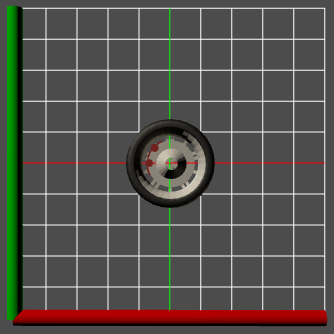
\includegraphics[width=0.9\textwidth]{../assets/wheel1.png}\\
    a)
  \end{minipage}
  \begin{minipage}{.5\textwidth}
    \centering
  	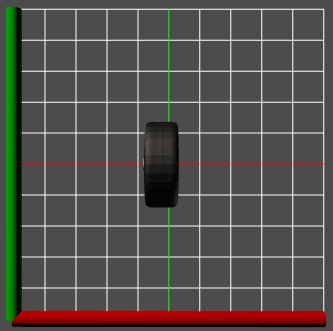
\includegraphics[width=0.9\textwidth]{../assets/wheel2.png}\\
    b)
  \end{minipage}\\
  \begin{minipage}{.5\textwidth}
    \centering
  	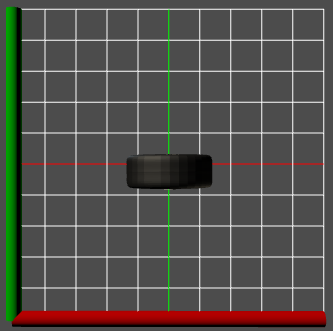
\includegraphics[width=0.9\textwidth]{../assets/wheel3.png}\\
    c)
  \end{minipage}
  \begin{minipage}{.5\textwidth}
    \centering
  	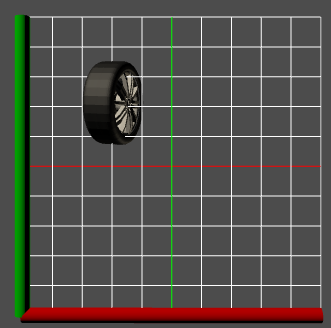
\includegraphics[width=0.9\textwidth]{../assets/wheel4.png}\\
    d)
  \end{minipage}
  \caption{Figures \ref{fig:wheel}a-c show common orientations the \gls{3D} model of a wheel could have. Figure \ref{fig:wheel}d shoes the worst case.}
	\label{fig:wheel}
\end{figure}

Figure \ref{fig:wheel} demonstrates multiple orientations a \gls{3D} model of a wheel can have. Figures \ref{fig:wheel}a-c are common
orientations, since it is disputable which of these could be considered the
norm. But if one depends on art from 3rd parties, the orientation and position
could be completely arbitrary like in Figure \ref{fig:wheel}d).

These properties could be added and adjusted via any text editor by opening the
generated \gls{X3D} file, but the resulting work-flow is not user-friendly. The
following list explains the work-flow using just a text editor.

\begin{enumerate*}
  \item Model the \gls{3D} application, including the \gls{3D} scene structure.
  \item Generate the \gls{3D} scene and the application code.
  \item Run the application and evaluate the scene and think about what objects need to go where and whether they need to be scaled.
  \item Type random translation, rotation and scale values into the transform nodes.
  \item Run the application again and evaluate whether the transformations are correct (since one does not know anything about the orientation of the object).
  \item Go back to 4. until all objects are placed correctly.
\end{enumerate*}

Tools like Maya or Blender could be used for this, but their import
and export filters discard important meta-data that is necessary for the
round-trip transformation. This is what \gls{SceGraToo} is meant to be. \gls{SceGraToo} addresses both of these issues. It allows for loading the root \gls{X3D} file and changing all transformations, containing the inline nodes,
using mouse interactions. For fine grained control \gls{SceGraToo} also
contains a tree view that allows the user to input exact attributes for
translations, rotations and scale (see Figure \ref{fig:tree-view}).

\subsection{Scope}\label{scope}

The provided application (\gls{SceGraToo}) addresses two issues:

\begin{enumerate*}
  \item Allowing the composition of generated \gls{X3D} scenes (with focus on usability). E.g., accompanying the \gls{3D} view, a tree view for fine grained editing, that should not only visualize the \gls{3D} scene's structure, but also allow for entering concrete coordinate values.
  \item During the editing process, the preservation of all information/meta-data must be guaranteed.
\end{enumerate*}
